\section{The Knower and the Known}


One of the fundamental differences between the Traditional and the modern worldviews regards the nature of knowing. For the modern mind, knowing depends on the thing known and the knower himself is passive. As far back as the Stoics, the analogy used was that of wax taking on the design of a seal; thus, the sense impressions in the mind are the effect of an external object. The moderns took this up again, although it then led to Kantian skepticism since there is no way to be sure the sense impression really matches the external object. On the other hand, those of a scientific bent totally ignored Kant and continued on their quest; this has consequences for the search for artificial intelligence and the Golem.

\begin{wrapfigure}{rt}{0.35\textwidth}
 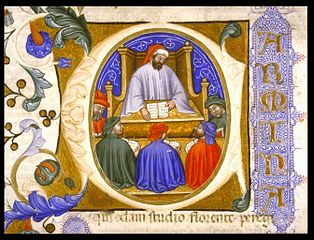
\includegraphics[scale=.5]{a20121023TheKnowerandtheKnown-img001.jpg}  
\end{wrapfigure}

In his Consolations of Philosophy, \textbf{Boethius} addresses the topic and rejects it:

\begin{quotex}
People think that the totality of their knowledge depends on the nature and capacity to be known of the objects of knowledge. But this is all wrong. \emph{Everything that is known is comprehended not according to its own nature, but according to the ability to know of those who do the knowing}. [my emphasis]

\end{quotex}
This needs to be pondered. It means that knowing is not an automatic process and that the object of knowledge does not reveal itself indiscriminately. For example, academics study Tradition as a set of texts that have appeared historically. The academic, then, believes that his impressions represent the truth of Tradition, and all he needs do is to catalog the texts and relate them, temporally or spatially.

But this is all wrong. Only the man who has prepared himself, who has developed within himself the ability to know, only he can understand Tradition. Boethius summarizes the stages of knowledge in the following schema; note, especially, how they relate to \textbf{Dante}'s four levels of understanding an esoteric text. Nothing in Tradition is arbitrary.

\begin{table}[h]\scriptsize
\begin{tabular}{cccc}\toprule 
Stage of knowledge &
Description &
Applies to &
Level of Interpretation\\\midrule
Sense Impression &
The senses examine shape as constituted in matter. &
Lower animals, plants &
Literal\\\midrule
Imagination &
Considers the shape apart from matter &
Higher animals &
Allegorical\\\midrule
Reason &
Transcends the imagination and reflects upon the species inherent in individual instances &
Man &
Moral\\\midrule
Intuition or Intelligence &
Passes beyond the sphere of the universe to behold the simple form itself with the pure vision of the mind. &
Divinity (God, angels, higher states of consciousness) &
Anagogical\\\bottomrule
\end{tabular}
\end{table}
Boethius elaborates:

\begin{quotex}
The point of greatest importance here is this: the superior manner of knowledge includes the inferior, but it is quite impossible for the inferior to rise to the superior. The senses cannot perceive anything beyond matter; imagination does not consider universal species; and reason does not comprehend simple form … [the Intellect] knows reason's knowledge of universals, imagination's knowledge of shape, and the sense's knowledge of matter without using reason, imagination, or the senses, but by the single glance of the mind according to the form.

\end{quotex}
Boethius makes clear that this is an active process:

\begin{quotex}
In perceiving corporeal phenomena the mind is not passively affected, but judges of its own power the experience subjected to the body.

\end{quotex}
This “power”, then, can be developed further and Boethius urges us on:

\begin{quotex}
Let us, then, if we can, raise ourselves up to the heights of that supreme intelligence. There reason will be able to see that which it cannot see by itself—it will be able to see how that which has no certain occurrence may be seen by a certain and fixed foreknowledge, \emph{a knowledge that is not opinion, but the boundless immediacy of the highest form of knowing}.

\end{quotex}
\paragraph{Golems and Artificial Intelligence}
The whole premise of the development of artificial intelligence is based on the passive reception of sense impressions. Since a computer can have no conception of the form of a cube, simple tasks, such as recognizing a box, are very difficult. Through sheer computational power, computers are, and will be, able to simulate intelligence, but not have intelligence in any real sense. Legends of golems and homunculi recognized this. The golem could not be merely a being or mechanism of matter; somehow it would have to be animated. In other legends, higher beings were invoked to animate a statue or a doll. But no one thought mere matter could display intelligence.


\hfill

I'm using the translation by V. E. Watts, published by Penguin Classics



\flrightit{Posted on 2012-10-23 by Cologero }

\begin{center}* * *\end{center}

\begin{footnotesize}\begin{sffamily}



\texttt{Logres on 2012-10-25 at 15:44 said: }

I wonder if Cassiodorus had similar knowledge – I am thinking he did, more than likely, given his career and task.


\hfill

\texttt{Cologero on 2012-10-26 at 12:28 said: }

Logres, Boethius was not breaking new ground, he thought the way intelligent men of the time did. (I'm excluding non-Traditional systems like stoicism or epicureanism.) It was that way for centuries; the Romance of the Rose and Chaucer both had high regard for Boethius. The “wonder” is why no one has similar knowledge today. For example, academic Chaucer scholars may pride themselves on their facility with Middle English. But can they truly understand Chaucer without grasping his worldview, from the inside, as it were? Why is that knowledge lost? Has it been disproved or simply lost?


\hfill

\texttt{Logres on 2012-10-26 at 21:30 said: }

In the Bagavad-Gita, Krishna tells Arjuna that there are lapses of knowledge, in which it sinks into nothingness, \& has to be renewed by direct intervention of an avatar. Can we still pull the ring out of the well? Did the ring hide itself?


\hfill

\texttt{Cassiodorus on 2012-10-28 at 23:06 said: }

“Has it been disproved or simply lost”.

That reminds of the first work I read by a defender of Tradition- Huston Smith's Forgotten Truth.


\end{sffamily}\end{footnotesize}
